% ------------------------------------------------------------------------------
% TYPO3 Version 10.4 - What's New (French Version)
%
% @license	Creative Commons BY-NC-SA 3.0
% @link		https://typo3.org/help/documentation/whats-new/
% @language	French
% ------------------------------------------------------------------------------

\section{Interface Utilisateur Backend}
\begin{frame}[fragile]
	\frametitle{Interface Utilisateur Backend}

	\begin{center}\huge{Chapitre 1~:}\end{center}
	\begin{center}\huge{\color{typo3darkgrey}\textbf{Interface Utilisateur Backend}}\end{center}

\end{frame}

% ------------------------------------------------------------------------------
% ...

\begin{frame}[fragile]
	\frametitle{Interface Utilisateur Backend}
	\framesubtitle{Ajustement de l'UI Backend}

	Légère altération de l'affichage de la colonne des modules backend.

	\begin{figure}
		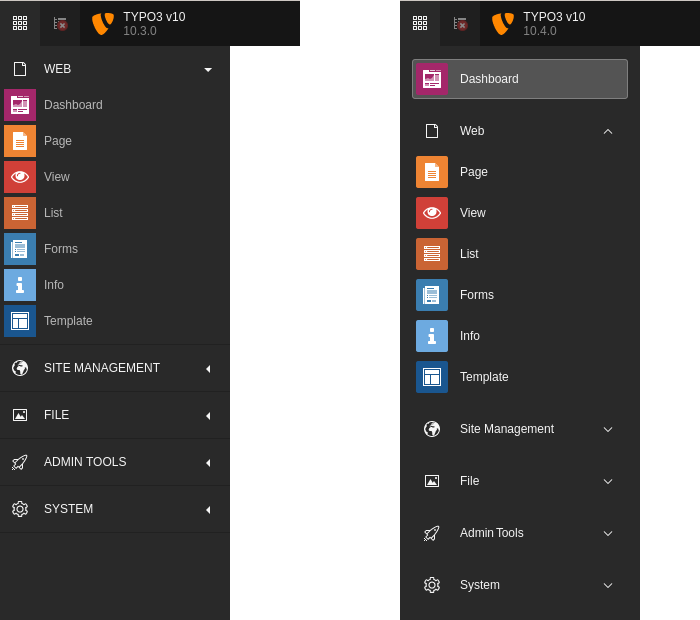
\includegraphics[width=0.5\linewidth]{BackendUserInterface/typo3-backend-ui.png}
	\end{figure}

\end{frame}

% ------------------------------------------------------------------------------
% Feature | 83128 | Content Element Filter

\begin{frame}[fragile]
	\frametitle{Interface Utilisateur Backend}
	\framesubtitle{Recherche dans Nouveau contenu}

	Lors de la création d'un contenu à l'aide de l'assistant «~Nouvel élément de contenu~»,
	l'utilisateur backend peut chercher le type de contenu~:

	\begin{figure}
		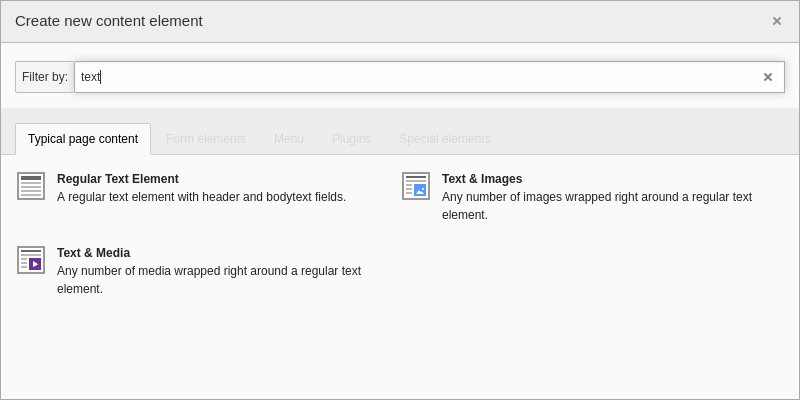
\includegraphics[width=0.6\linewidth]{BackendUserInterface/83128-ContentElementFilter.png}
	\end{figure}

\end{frame}

% ------------------------------------------------------------------------------
% Feature | 89513 | Provide password recovery for backend users

\begin{frame}[fragile]
	\frametitle{Interface Utilisateur Backend}
	\framesubtitle{Récupération du mot de passe}

	Les utilisateurs backend peuvent réinitialiser leur mot de passe en cas d'oubli.

	\begin{figure}
		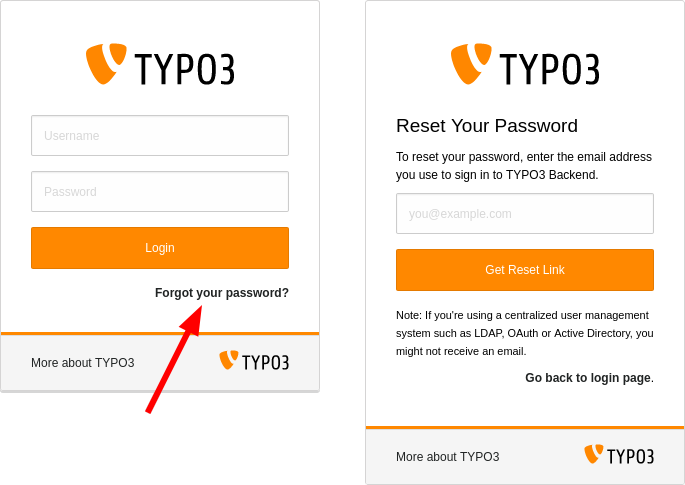
\includegraphics[width=0.6\linewidth]{BackendUserInterface/89513-ProvidePasswordRecoveryForBackendUsers.png}
	\end{figure}

\end{frame}

% ------------------------------------------------------------------------------
